\documentclass[14pt]{exam}
\usepackage[utf8]{inputenc}
\usepackage[T1]{fontenc}
\usepackage[spanish]{babel}
\usepackage[autostyle,spanish=mexican]{csquotes}
\usepackage{amsmath}
\usepackage{amsthm}
\usepackage{physics}
\usepackage{tikz}
\usepackage{float}
\usepackage[per-mode=symbol]{siunitx}
\usepackage{gensymb}
\usepackage{multicol}
\usepackage{chemformula}
\usepackage[left=2.00cm, right=2.00cm, top=2.00cm, 
     bottom=2.00cm]{geometry}

\usepackage[fontsize=14pt]{scrextend}
\usepackage{anyfontsize}
\usepackage{pgfplots}
\pgfplotsset{compat=1.8}

\renewcommand{\questionlabel}{\thequestion)}
\decimalpoint
\sisetup{bracket-numbers = false}


\title{\vspace*{-2cm}Examen de Repaso\vspace{-5ex}}
\date{\today}

\footer{}{\thepage}{}

\begin{document}
\maketitle

\section{Matemáticas.}

\begin{questions}

\question Selecciona el valor de $x$ e $y$ que se obtienen al resolver el siguiente sistema de ecuaciones de primer grado:
\begin{align*}
\begin{cases}
10 \, x - 3 \, y = 36 \\
2 \, x + 5 \, y = -4
\end{cases}
\end{align*}
\\[0.5em]
\begin{oneparchoices}
    \choice $x = 0$, $y = 1$. 
    \choice $x = 1$, $y = 2$. 
    \choice $x = 3$, $y = -2$. 
    \choice $x = -3$, $y = 2$. 
\end{oneparchoices}
\question Yuya tenía cierta suma de dinero. Gastó $\$30$ en libros y los $\dfrac{3}{4}$ de lo que le quedaba después del gasto anterior los ocupó en ropa. Si le restan $\$30$. ¿Cuánto dinero tenía al principio?
\\[0.5em]
\begin{oneparchoices}
    \choice $\$120$
    \choice $\$150$
    \choice $\$180$
    \choice $\$90$
\end{oneparchoices}
\question ¿Cuál de las siguientes gráficas representa la expresión $x + y = 5$
\\[0.5em]
\begin{minipage}{0.4\linewidth}
\begin{figure}[H]
    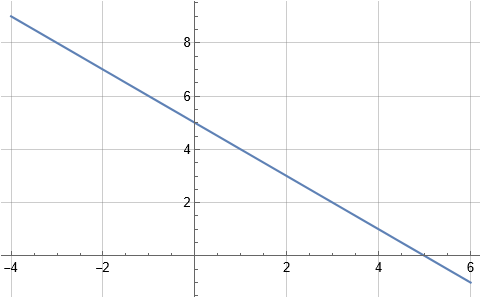
\includegraphics[scale=0.5]{Imagenes/Examen_Repaso_2023_03_07_01.png}
    \caption{A}
\end{figure}
\end{minipage}
\begin{minipage}{0.4\linewidth}
\begin{figure}[H]
    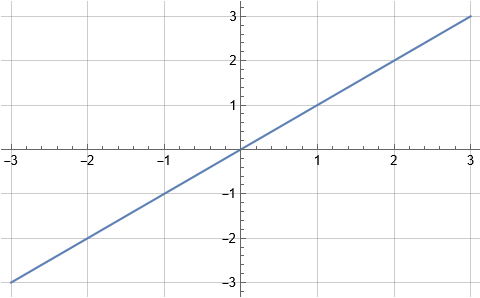
\includegraphics[scale=0.5]{Imagenes/Examen_Repaso_2023_03_07_02.png}
    \caption{B}
\end{figure}
\end{minipage}
\\
\begin{minipage}{0.4\linewidth}
\begin{figure}[H]
    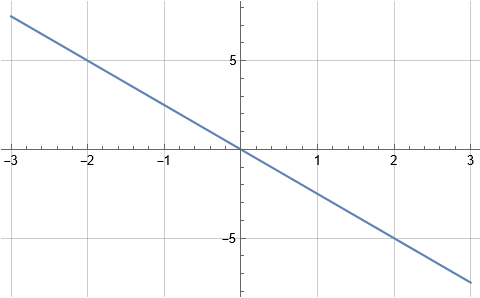
\includegraphics[scale=0.5]{Imagenes/Examen_Repaso_2023_03_07_03.png}
    \caption{C}
\end{figure}
\end{minipage}
\begin{minipage}{0.4\linewidth}
\begin{figure}[H]
    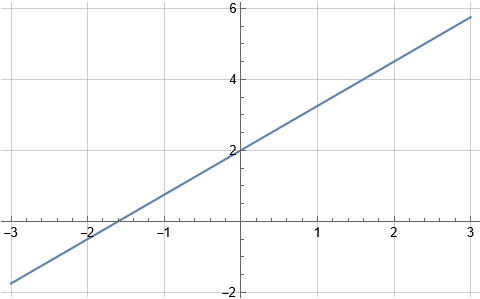
\includegraphics[scale=0.5]{Imagenes/Examen_Repaso_2023_03_07_04.png}
    \caption{D}
\end{figure}
\end{minipage}
\question ¿Cuál es la raíz cuadrada de $\sqrt{64 x^{8} y^{10}}$ \quad?
\\[0.5em]
\begin{oneparchoices}
    \choice $8 x y^{2}$
    \choice $8 x^{4} y^{6}$
    \choice $8 x^{4} y^{5}$
    \choice $-8 x^{4} y^{5}$
\end{oneparchoices}
\question ¿Cuál es la raíz cuadrada de $\sqrt{\dfrac{20}{25}}$ \quad?
\\[0.5em]
\begin{oneparchoices}
    \choice $\dfrac{5 \sqrt{5}}{2}$
    \choice $\dfrac{3 \sqrt{5}}{5}$
    \choice $\dfrac{7 \sqrt{5}}{5}$
    \choice $\dfrac{2 \sqrt{5}}{5}$
\end{oneparchoices}
\end{questions}

\section{Física.}

\begin{questions}
    \question Si la velocidad del tren bala es de $\SI{603}{\kilo\meter\per\hour}$. ¿Qué distancia ha recorrido en $\SI{1}{\minute}$?
    \\[0.5em]
    \begin{oneparchoices}
        \choice $\SI{11050}{\meter}$
        \choice $\SI{10015}{\meter}$
        \choice $\SI{10050}{\meter}$
        \choice $\SI{10055}{\meter}$
    \end{oneparchoices}
    \question El corredor jamaicano Usain Bolt estableció el récord de velocidad en la carrera de $\SI{100}{\meter}$ con un tiempo de $\SI{9.58}{\second}$. ¿Cuál fue su velocidad expresada en $\SI{}{\kilo\meter\per\hour}$?    \\[0.5em]
    \begin{oneparchoices}
        \choice $\SI{35.70}{\kilo\meter\per\hour}$
        \choice $\SI{37.57}{\kilo\meter\per\hour}$
        \choice $\SI{35.77}{\kilo\meter\per\hour}$
        \choice $\SI{38.80}{\kilo\meter\per\hour}$
    \end{oneparchoices}
    \question La moto Ducatti Superleggera V4 corre a un máximo de $200$ millas por hora. A la máxima velocidad, ¿cuánto tiempo (en segundos) tarda en recorrer $\SI{350}{\meter}$?
    \\[0.5em]
    \begin{oneparchoices}
        \choice $\SI{3.854}{\second}$
        \choice $\SI{3.914}{\second}$
        \choice $\SI{4.314}{\second}$
        \choice $\SI{5.869}{\second}$
    \end{oneparchoices}
    \question Durante la clase un alumno no alcanzó a anotar debidamente una expresión, lo que anotó fue lo siguiente: $= \dfrac{v_{f} - v_{i}}{t}$. Es posible identificar la variable que le hace falta a la expresión, pero ¿qué tipo de unidades le corresponden? Justifica tu respuesta.
    \\[0.5em]
    \begin{oneparchoices}
        \choice $\SI{}{\meter\per\second}$
        \choice $\SI{}{\square\meter\per\square\second}$
        \choice $\SI{}{\meter\per\square\second}$
        \choice $\SI{}{\square\meter\per\second}$
    \end{oneparchoices}
    \newpage
    \question Se grafica la velocidad de un objeto con respecto al tiempo como se muestra a continuación: ¿Cuál es la aceleración de ese objeto? Justifica tu respuesta.
    \begin{figure}[H]
        \centering
        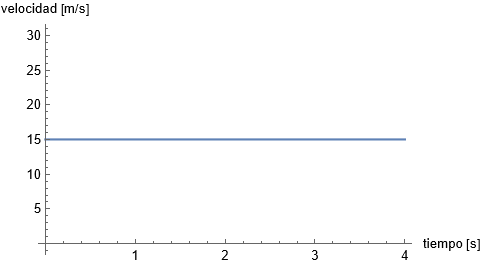
\includegraphics[scale=0.7]{Imagenes/Examen_Repaso_2023_03_07_05.png}
    \end{figure}
    \begin{oneparchoices}
        \choice $\SI{0}{\meter\per\square\second}$
        \choice $\SI{15}{\meter\per\square\second}$
        \choice $\SI{15}{\square\meter\per\square\second}$
        \choice $\SI{-15}{\meter\per\square\second}$
    \end{oneparchoices}
    
\end{questions}
\end{document}